\documentclass[12pt,twoside,a4paper]{article}
\usepackage[utf8]{inputenc}
\usepackage[english,german]{babel}
\usepackage{utopia}
\usepackage[margin=1in]{geometry}
\usepackage[parfill]{parskip}
\usepackage{makeidx}
\usepackage[onehalfspacing]{setspace}
\usepackage{fancyhdr}
\usepackage{lastpage}
\usepackage{hyperref}
\usepackage{graphicx}
\renewcommand{\sffamily}{phv}

\newcommand{\titleText}{Modul 153 Projekt\\\textbf{Anti-Social}}
\newcommand{\authorText}{T. Bonomelli, P. Günthard}
\newcommand{\dateText}{\today}

\title{\titleText}
\author{\authorText}
\date{\dateText}

\pagestyle{fancy}
\fancyhf{}

\fancyhead[EL]{\titleText}
\fancyhead[OR]{\today\\\textbf{\authorText}}
\cfoot{\thepage \space von \pageref{LastPage}}

\begin{document}
	\maketitle
	\tableofcontents
	\section {Projektbeschrieb}
	
	\subsection{Ausgangslage}
	
	Die Ausgangslage des Projektes ist ein Auftrag bei dem eine Datenbank entwickelt werden muss. Die Datenbank muss gewissen Vorgaben entsprechen, so sollte sie mindestens 15 Entitäten enthalten und allen Normalformen entsprechen.
	
	\subsection{Beschreibung}
	
	Unsere Datenbank soll eine Art soziales Netzwerk abbilden. In diesem sozialen Netzwerk kann man:
	\begin{itemize}
		\item Account erstellen
		\item Account löschen
		\item Berechtigungen / Rollen für Account erteilen resp. enziehen.
		\item Post erstellen
		\item Post löschen
		\item Account Status setzen
		\item Kommentar setzen
		\item Kommentar löschen
		\item Post typ setzen
		\item Post liken
		\item Post tagen
		\item Gruppe erstellen
		\item Account einer Gruppe beitreten
		\item Account Gruppe verlassen
		\item Gruppe löschen
		
	\end{itemize}
	
	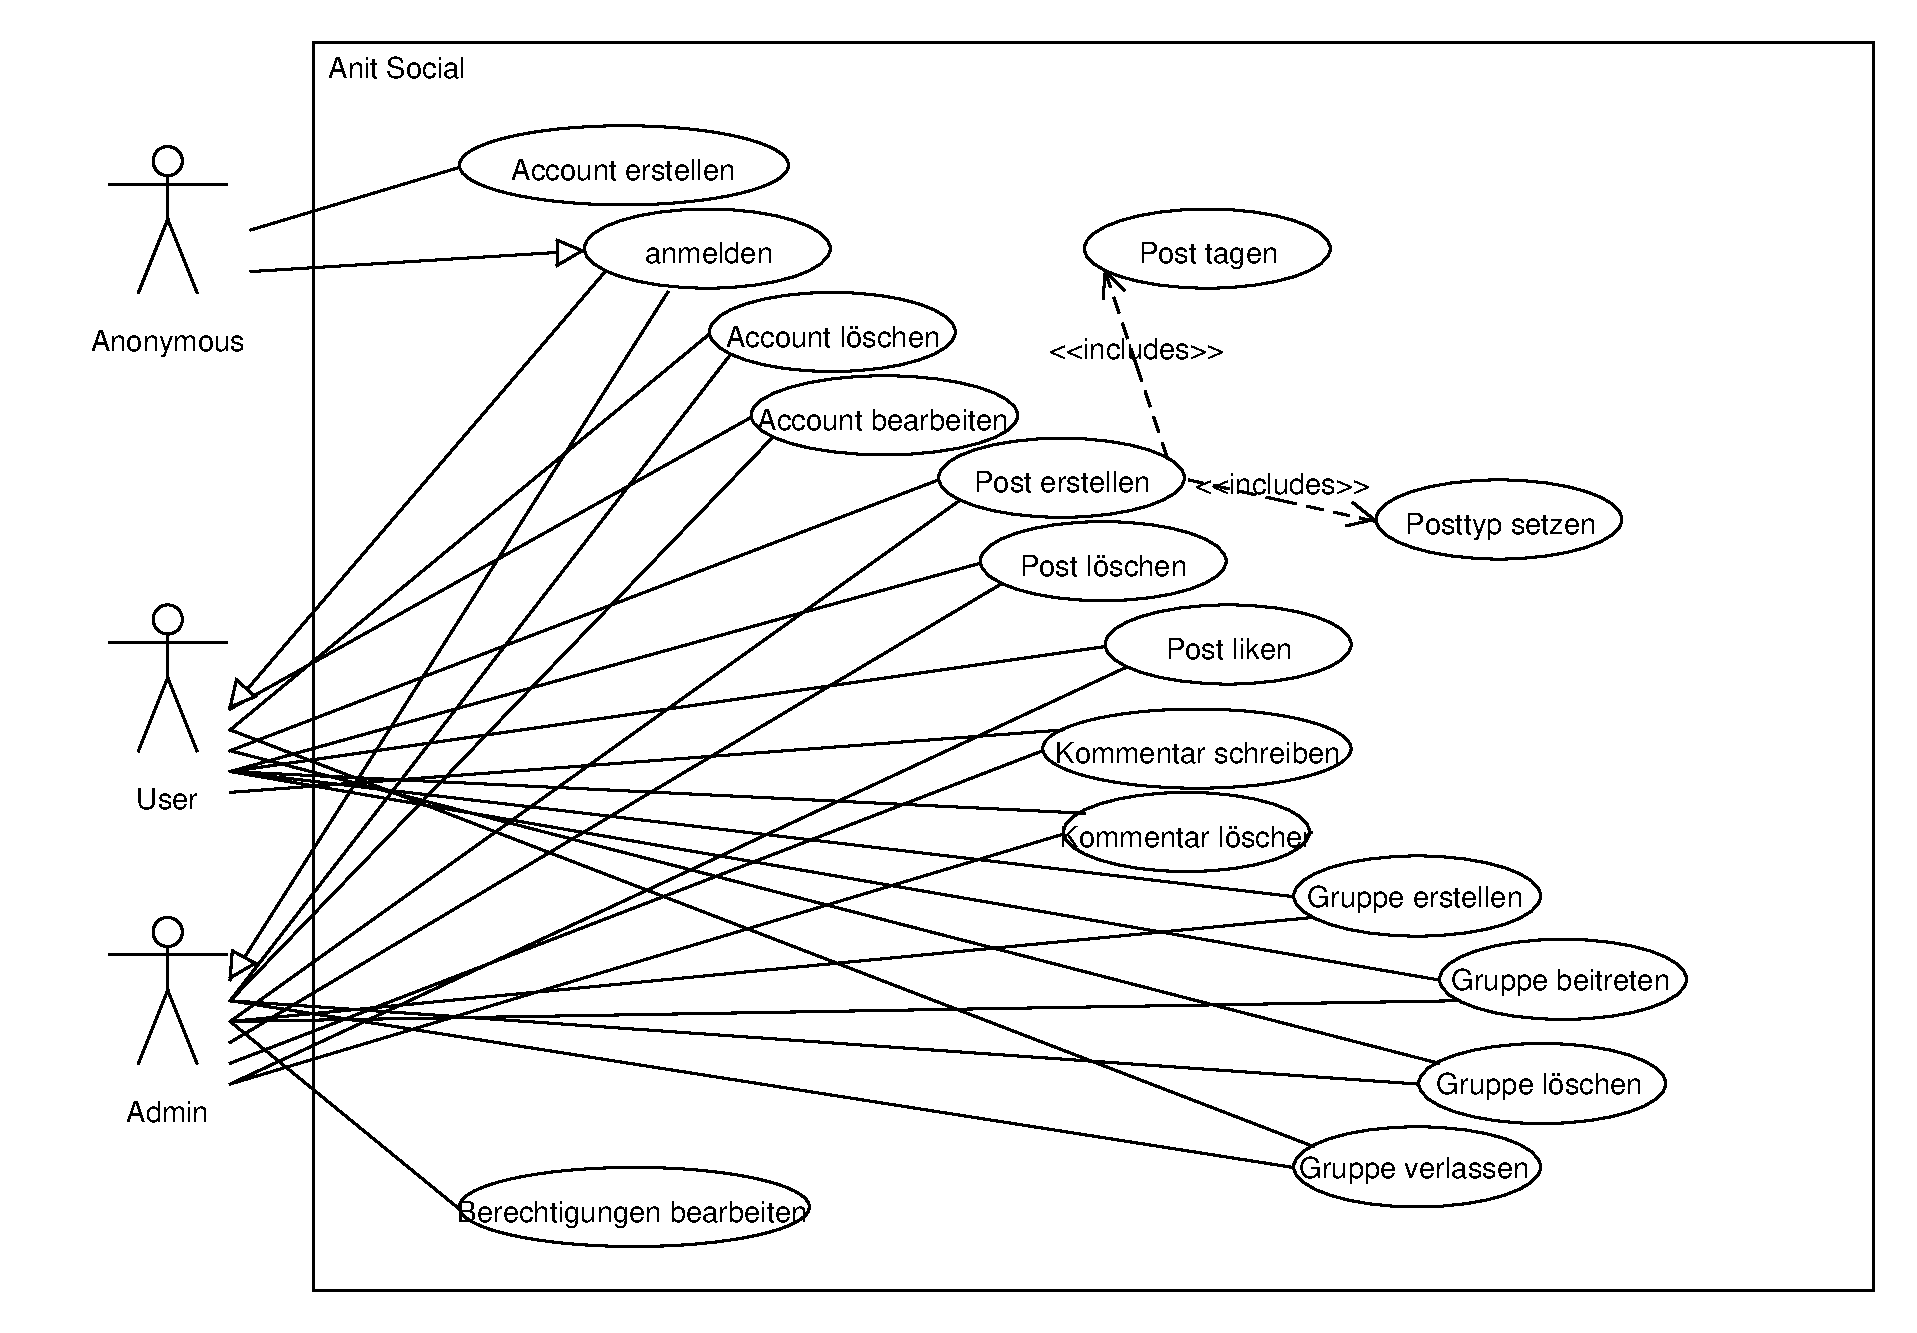
\includegraphics[width=15cm]{ucprj}
	
	\section{Logisches ERD}
	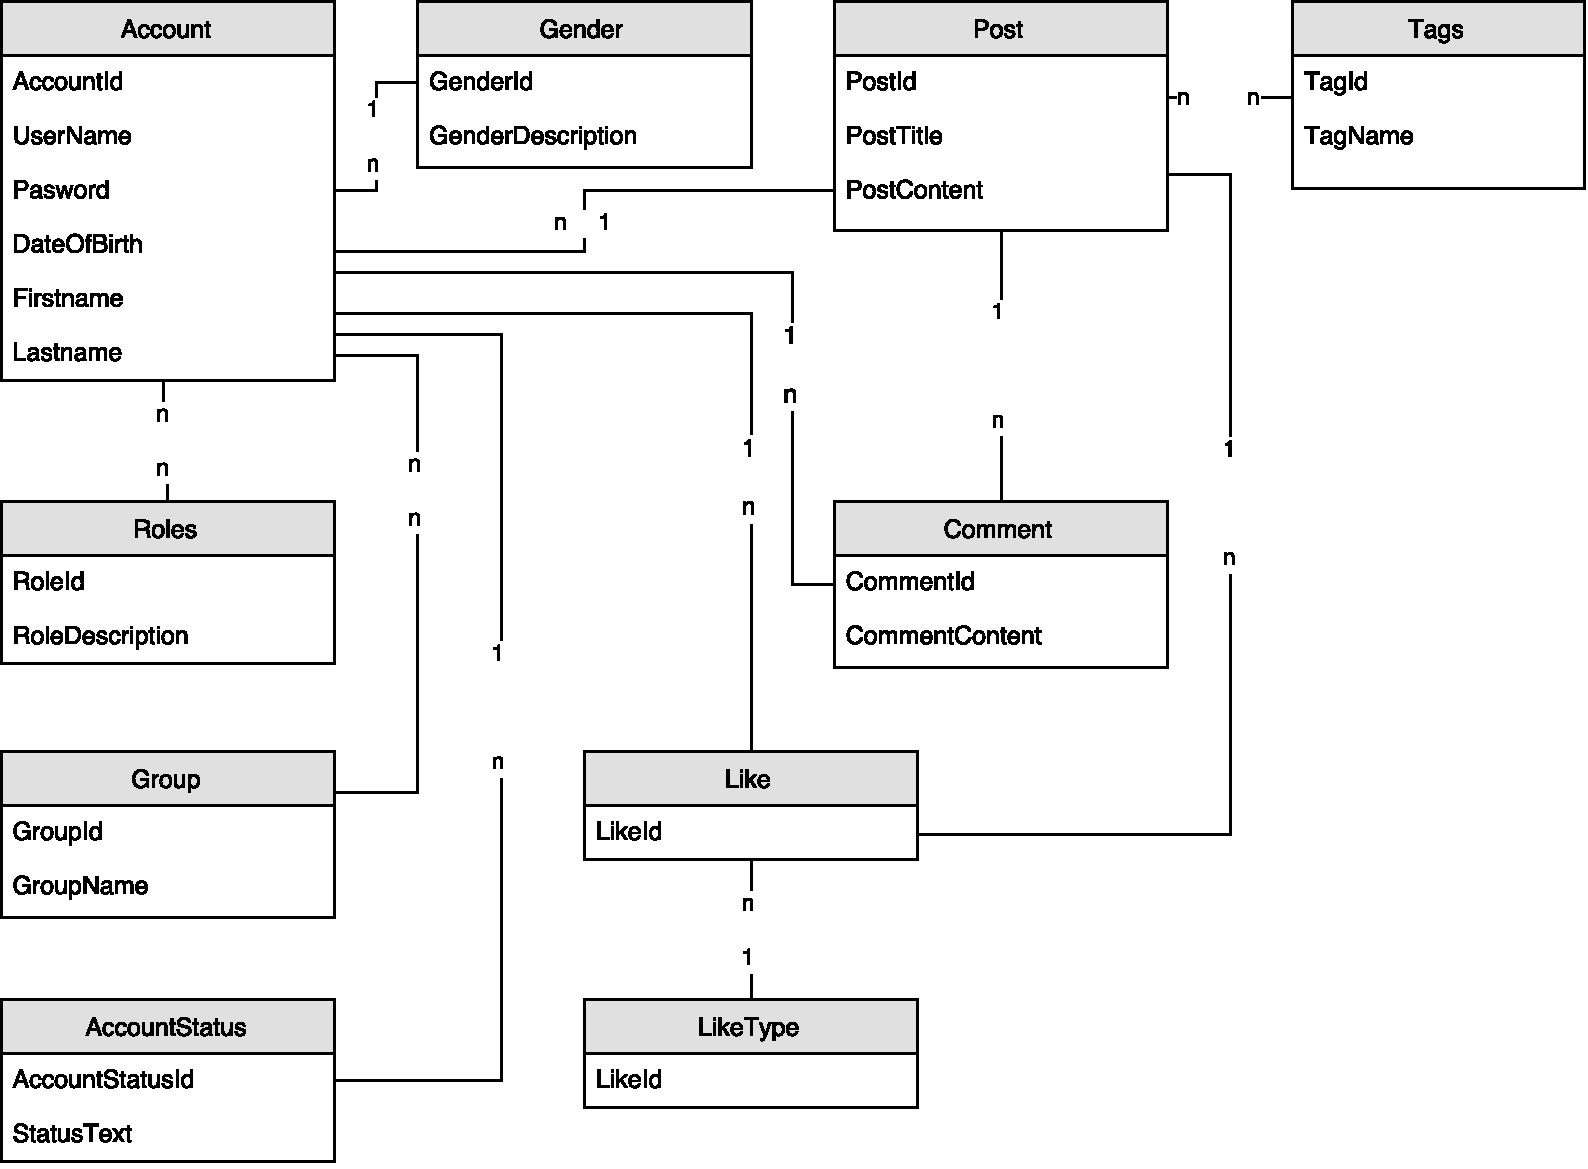
\includegraphics[width=15cm]{erd_a}
	
	
	
\end{document}